\chapter{Implementation}
\label{ch:implementation}
This chapter presents the technical implementation of the dynamic and heterogeneous crowd computing platform in detail. The implementation leverages modern web technologies introduced in chapter \ref{ch:methodology} to create a high-performance distributed computing solution for the web. At its core, the system utilizes WebAssembly for cross-platform compatibility, high performance, and language independence (\ref{sec:methodology:wasm}), WebSockets for efficient bidirectional communication (\ref{sec:methodology:websokets}), and WebWorkers for potential parallel Task execution (\ref{sec:methodology:webworker}).

The following sections describe the components of the architecture, communication sequences, scheduling strategies, persistence mechanisms and the challenges encountered during the implementation phase. Sections \ref{sec:implementation:backend} and \ref{sec:implementation:frontend} describe the interaction with the platforms API and web interface.

\section{Architecture}
\label{sec:implementation:architecture}
\begin{figure}[htbp]
    \centering
    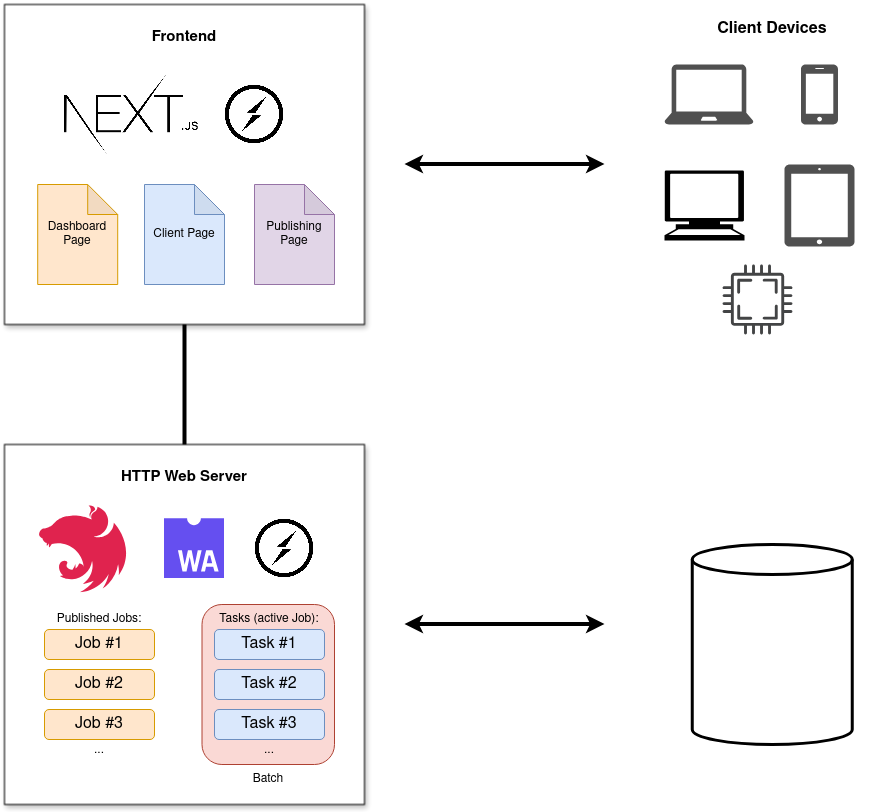
\includegraphics[width=0.95\textwidth]{gfx/figures/WebAssembly-MA.png}
    \caption{Architecture Modell of the platform}
    \label{fig:implementation:architecture}
\end{figure}

The platform consists of the following three components:
\begin{itemize}
    \item Server (Backend) as the central component handling the distribution of Tasks and persistence of Job results \ref{sec:implementation:backend}, implemented using Nest.js \cite{methodology:nestjs}
    \item Frontend providing the web application for all clients \ref{sec:implementation:frontend}, implemented using Next.js \cite{methodology:nextjs}
    \item Database for persisting Job and User data, implemented with PostgreSQL \cite{methodology:db}
\end{itemize}

Figure \ref{fig:implementation:architecture} illustrates the architecture of the platform. Heterogenous clients, diverse in hardware and operating system, are able to connect to the platform. Clients access the platform throuh the Frontend which than establishes the WebSocket communication with the Server using the Socket.IO \cite{methodology:websockets2} library. Each client (Worker and Administrator) maintains a bidirectional WebSocket connection to the Server. The database is exclusively accessible by the Server.

\subsection{Communication}
\label{subsec:implementation:architecture:communication}
When clients establish a connection to the platform by accessing the frontend application, a WebSocket connection is initiated. This enables real-time and bidirectional communication between the Server and client. Therefore this connection is used to send Tasks from the Server to the Workers as well to send the result of each Tasks from the Workers back to the Server. Furthermore, Administrators receive real-time data about all connected Workers and the current status of each Job through this WebSocket connection.

\begin{figure}[htbp]
    \centering
    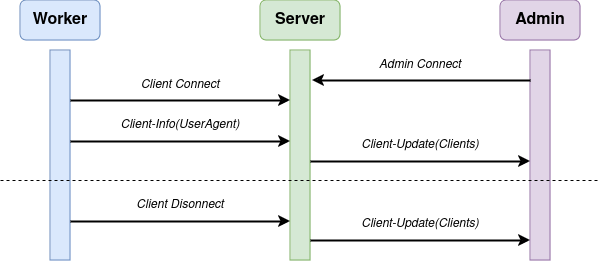
\includegraphics[width=0.95\textwidth]{gfx/figures/communication-connection.png}
    \caption{Communication: Connection of Worker \& real-time Update for Administrator}
    \label{fig:implementation:communication1}
\end{figure}

Figure \ref{fig:implementation:communication1} illustrates the process of a Worker connecting to the Server. Upon successful connection, the Worker transmits all available information regarding its hardware and operating system in form of the Browser User Agent to the Server. After this initialization of the Worker, all previously connected Administrators automatically receive an updated list of all connected Workers. Similarly, if a Worker disconnects a automatic update is send to all Administrators.

\begin{figure}[htbp]
    \centering
    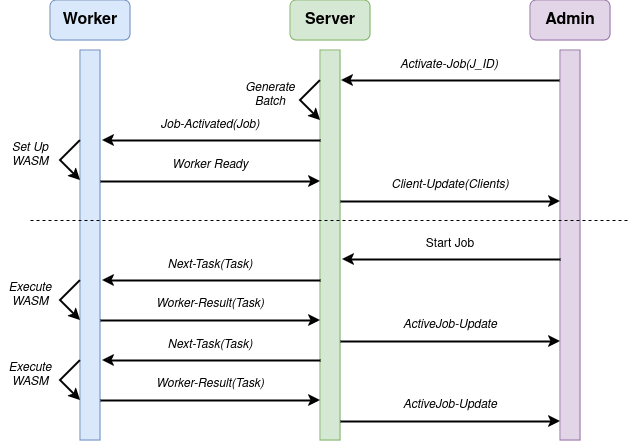
\includegraphics[width=0.95\textwidth]{gfx/figures/communication-jobexecution.png}
    \caption{Communication: Administrator starts Job \& Worker executes Tasks}
    \label{fig:implementation:communication2}
\end{figure}

Figure \ref{fig:implementation:communication2} illustrates the Job initiation and execution process. The sequence begins when an Administrator changes a Jobs status to \emph{ACTIVE}. The Server then generates a Batch of Tasks for the specified Job and notifies all connected Workers by transmitting the activated Job to them. Upon receiving this notification, each Worker retrieves the corresponding WebAssembly binary from the Server and initializes a WebWorker with the WebAssembly environment for this active Job. When this step is successfully completed the Worker notifies the Server which sets the Workers \emph{ready} attribute to true. This update is also forwarded to all Administrators.

If an Administrator changes the status of a active Job to \emph{RUNNING}, the Server than distributes unique Tasks from the current Batch to all Workers that have transmitted the \emph{Worker Ready} message and therfore have successfully completed the Job initialization process. Each Worker executes its assigned Task, then appends the corresponding result to the Task object, and transmits the completed Task back to the Server. If unprocessed or unscheduled Tasks remain in the Batch at the moment of receiving the completed Task, the Server responds by assigning the next pending Task to this Worker. Additionally, the Server notifies all Administrators after each successfully completed Task. This enables monitoring of the Jobs progression in real-time for all Administrators.

If a Worker is connecting while there is already an active or running Job, the communication sequence is automatically executed identically. Accordingly the Worker starts to initializes this Job and then proceeds to process Tasks of the Batch, hence enabling dynamic participation in ongoing Jobs for Workers.

\begin{figure}[htbp]
    \centering
    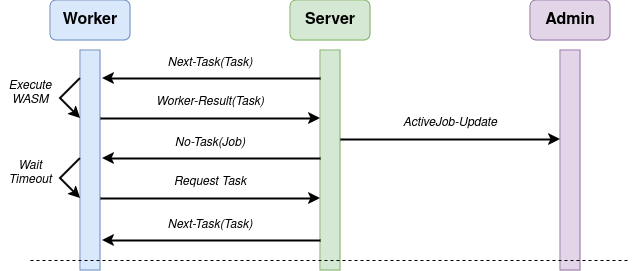
\includegraphics[width=0.95\textwidth]{gfx/figures/communication-timeout.png}
    \caption{Communication: Rescheduling of Tasks after timeout}
    \label{fig:implementation:communication3}
\end{figure}

Each Job has a timeout attribute for its Tasks. Scheduled Tasks that remain incomplete after their allocated timeout period can be redistributed to a different Worker. This mechanism enables the rescheduling of Tasks, which have been assigned to a malfunctioning Worker or a Worker that has disconnected before completing its assigned Task. Additionally, this approach allows rescheduling of Tasks that have been assigned to slower Workers, known as Stragglers, to more efficient Workers. Hence this mechanism can optimize the overall execution time of a Job.

Figure \ref{fig:implementation:communication3} illustrates the case, if all Tasks of the Batch already have been scheduled, but one or more are not yet completed. When a Worker transmits a completed Task to the Server while the timeout period of all other scheduled Tasks has not expired, the Server responds with the \emph{No-Task} message accompanied by the Job object of the currently active Job. The Worker extracts the status and the timeout value from this Job objects and initiates a waiting period equivalent to the timeout value plus a randomized overhead, if the Jobs status is still \emph{RUNNING}. This additional randomized overhead time prevents simultaneous Task requests, if multiple Workers are waiting for a Task at the same time. After the completion of the waiting period, the Worker transmits a \emph{Request Task} message to the Server. The server responds either with a newly available Task or another \emph{No-Task} message, repeating this sequence until the current Batch is fully processed.

\subsection{Persistence}
\label{subsec:implementation:architecture:persistence}
This section describes the persistent data storage implementation of the platform. The primary adressed objective is to ensure system recovery capabilities in cases of system failures, unexpected system crashes, or scheduled system restarts.

The following data objects have been identified as critical for a system recovery:
\begin{itemize}
    \item Job data
    \item Task input arguments
    \item Task results
    \item User credentials
\end{itemize}
Information regarding Workers, their hardware specifications and operating systems is intentionally excluded from permanent storage.

The system implements a robust persistence mechanism for Job progression. When a running Job is stoped, the current progress and all Task results are automatically saved, hence actively stoping a running Job initiates the persistence process for this Job's current state. This functionality should be utilized if the platform is scheduled to be restarted or terminated.

Additionally the system persists Job progress after each Batch completion. This mechanism enables periodic Job backups, as each Batch completion establishes a save point. Consequently, the Batch size determines the Job's fallback tolerance in the event of an unexpected system failure.

It is noteworthy that from a Worker's perspective, tasks cannot be persisted. Since WebAssembly is executed in a save sandbox environment the code has usually no access to local files. In the event of an unexpected crash of the Worker's WebAssembly process or browser, the progress of the affected Task will be lost.

\subsubsection{Database}
The PostgreSQL database is used to store the User credentials aswell as each Job object. Each Job object contains a progress attribute that represents a pointer indexing the last completed Task in the Task sequence. During Job recovery, this progress value determines the starting point for the first Task in the new Batch.

\subsubsection{Data in Files}
The system utilizes text files for persistent storage of Task input arguments and Task results. Each Job's critical information about its Tasks is stored in a separate text file for input arguments and the results. 

The method to generate a Batch reads the Task input arguments text file line by line, where each line represents an input argument. For each line, the system creates a unique Task and adds it to the Batch in sequence.

When the progress of a Job is persisted, the Server writes the results of all completed Tasks within the Batch to the Task results text file. Each result is written in a new line, and the results are stored in sequential order.

Additionally the Server implements a special handling mechanism for Tasks that produce files as results. When a Worker transmits such a completed Task, the Server immediately stores the result file in a result directory corresponding to the running Job. Subsequently, when later a Jobs progress is saved, the Server stores the file path to each result in the corresponding Task results text file instead of the actual result data.

\subsection{Scheduling}
\label{subsec:implementation:architecture:scheduling}
The Server is responsible for distributing Tasks from the current Batch to participating Workers. To maximize performance, the Server keeps track of scheduled Tasks to prevent duplicate Task distribution among Workers. The scheduling of Tasks follows the \ac{FIFO} methodology, scheduling the Tasks in sequential order. As described in Section \ref{subsec:implementation:architecture:communication}, each Job entity has a timeout attribute for its Tasks. Only if a Task remains incomplete after its designated timeout period has expired can this Task be rescheduled. This mechanism serves to mitigate issues arising from malfunctioning, disconnected, or straggling Workers.

The scheduling mechanism could be enhanced through the implementation of performance-aware distribution, allocating computationally intensive Tasks to Workers identified as having superior hardware.

\subsection{Security through Authentication \& Authorization}
\label{subsec:implementation:authentication}
To prevent malicious use, particularly in critical processes managed by Administrators, the system implements a authentication mechanism. This is achieved through User credentials combined with a \ac{JWT}.

Authentication and Authorization are two key security concepts that work together to protect systems and data. Authentication is used to verify a clients identity - proving they are who they claim to be - in this platform realized through User credentials. Once a User is authenticated, Authorization determines what they're allowed to do within the system by checking their permissions and access rights. The \emph{userRole} attribute in the user object defines the specific access permissions. Together, these processes ensure that not only are Users verified, but they can only access the resources and perform the actions appropriate for their role or permission level.

A \ac{JWT} implements a compact, URL-safe methodology for secure information transmission between parties as a \acs{JSON} object \cite{implementation:jwt}. The token architecture comprises three dot-separated components: a header that describes the token type and signing algorithm, a payload containing the encoded data, and a signature to verify the token's authenticity \cite{implementation:jwt}. \ac{JWT}s are commonly used in authentication and authorization processes, where information like user identity and permissions needs to be securely shared between services. The token can be verified by other services using the signature, eliminating the need to repeatedly validate credentials against a database. This makes \ac{JWT}s particularly useful in modern web applications and microservices architectures where secure, stateless authentication is required. \cite{implementation:jwt}

Upon successful User authentication, when a client connects to the platform, the Server generates and sings a \ac{JWT}, which is used to authenticates subsequent requests of this User. This generated \ac{JWT} is stored as a browser cookie on the client side which remains valid during a two-day expiration period. The data stored in the \ac{JWT} payload is a \acs{JSON} object containing the attributes \emph{id}, \emph{name}, and \emph{userRole} corresponding to the authenticated User. Clients transmitt their specific \ac{JWT} with every \ac{API} request or when establishing a WebSocket connection. Hence the Server can then use this token to authenticate the User and check if the User is authorized for this action.

\section{Backend}
\label{sec:implementation:backend}
This section describes the usage and features of the Backend, which is implemented using the NestJS framework. The Backend application serves three primary functions: 

\begin{itemize}
    \item Data management for Users, Jobs, Tasks, and their associated results.
    \item Handling the WebSockets communication with all connected clients.
    \item Task distribution to participating Workers.
\end{itemize}

Therefore the Backend implementation represents the Server component described in subsection \ref{subsec:methodology:entities:Server}.

To manage and interact with Jobs or Users, the Backend exposes multiple endpoints through a \acs{REST}ful \ac{API}. Figure \ref{fig:implementation:backend} presents a list of all available endpoints and their corresponding \acs{HTTP} request method. Due to their handling of critical and sensitive data, all endpoints are secured through \ac{JWT} authorization and require Administrator privileges, granted only for Users with the Admin \emph{userRole}. The login endpoint represents the only exception to this security measure, as it serves to generate a \ac{JWT} in the first place by validating a Users credentials, and therefore operates without any \ac{JWT} authorization.

\begin{figure}[bth]
    \myfloatalign
    \subfloat[Job \ac{API} endpoints]{
    \label{fig:implementation:backend:job}
    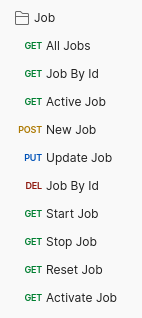
\includegraphics[width=.25\linewidth]{gfx/figures/Job_API.png}
    } \quad \quad
    \subfloat[User \ac{API} endpoints]{
    \label{fig:implementation:backend:user}
    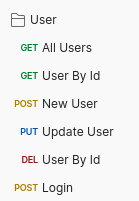
\includegraphics[width=.25\linewidth]{gfx/figures/User_API.png}
    }
    \caption{Available Backend \ac{API} endpoints}
    \label{fig:implementation:backend}
\end{figure}

The Backend \ac{API} implements comprehensive \ac{CRUD} operations for both Job and User entities. These endpoints enable the retrieval of individual entities or complete entity collections, the creation of new entities, and the modification or removal of existing entities.

Furthermore the \ac{API} exposes four additional endpoints to change the sate of Jobs and therefore providing the features to control Job execution with the platform. Upon Job activation, a Batch associated to this Job is generated and all connected Workers are triggered to initiate the initialization of their WebAssembly environment. Starting a Job initiates the process of distributing Tasks from its Batch to \emph{ready} and participating Workers. When a Job is stopped, its current state is persisted in the Server as described in subsection \ref{subsec:implementation:architecture:persistence}. The reset operation permanently removes all progress associated with a Job and generates a new unprocessed Batch containing the initial Tasks.

Additionally the Backend \ac{API} serves static files of the compiled WebAssembly binaries and the optionally required JavaScript gluecode files of each Job. These files are required to initializes a WebAssembly environment, and are therfore requested by Worker nodes.

Furthermore the Backend implements a WebSocket-based communication protocol as described in subsection \ref{subsec:implementation:architecture:communication} that manages bidirectional data streams between the Server and connected client nodes. This implementation enables performant Task distribution and Task result collection as well as real-time comunication for Job progress monitoring while minimizing the overall communication overhead.

\section{Frontend}
\label{sec:implementation:frontend}
This section describes the features and main web pages served by the Frontend. It is implemented utilizing the NextJS framework in combination with styled components from the React Bootstrab library \cite{implementation:bootstrap}. The core features implemented in the Frontend application are:

\begin{itemize}
    \item Providing an easy to use interface to interact with the platform.
    \item Establishing a WebSocket connection to the Server.
    \item Executing WebAssembly in a WebWorker.
    \item Serving a dashboard to manage Jobs.
\end{itemize}

The Frontend implements two main web pages. These are the \emph{Dashboard Page} and the \emph{Client Page}.

\subsection{Dashboard Page}
\label{subsec:implementation:dashboard-page}

The \emph{Dashboard Page}, displayed in figure \ref{fig:implementation:dashboard-page}, is only accessible for Administrators. This page is used to monitor all connected Workers and the progress of Jobs in real-time. Furthermore are Administrator able to manage Jobs through this web page.

\begin{figure}[ht!]
    \myfloatalign
    \subfloat[Dashboard Page: Job List]{
    \label{fig:implementation:job-list}
    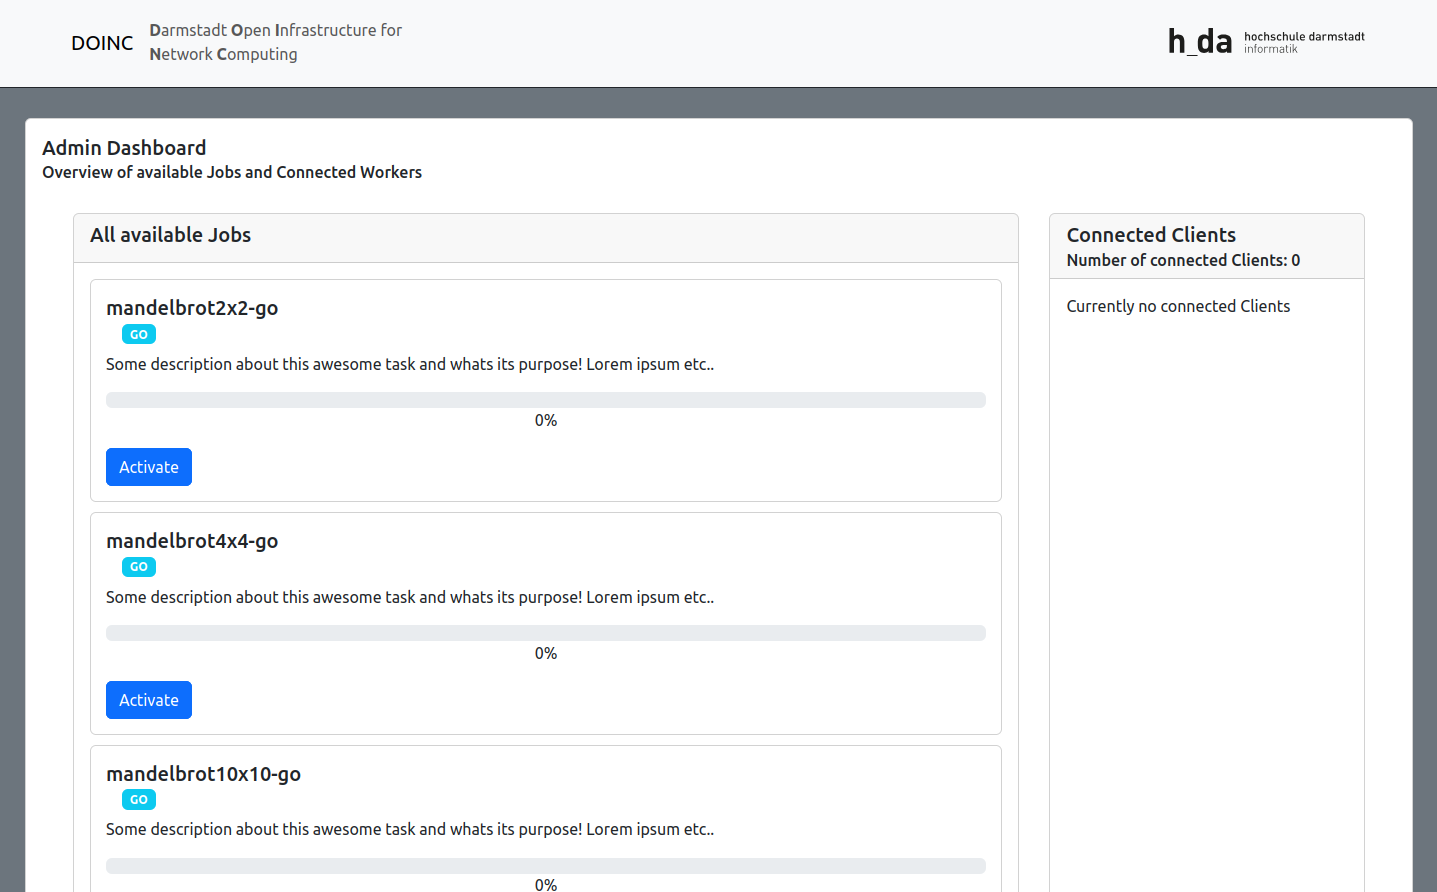
\includegraphics[width=.95\linewidth]{gfx/figures/job-list.png}
    } \\
    \subfloat[Dashboard Page: Active Job (TODO)]{
    \label{fig:implementation:active-job}
    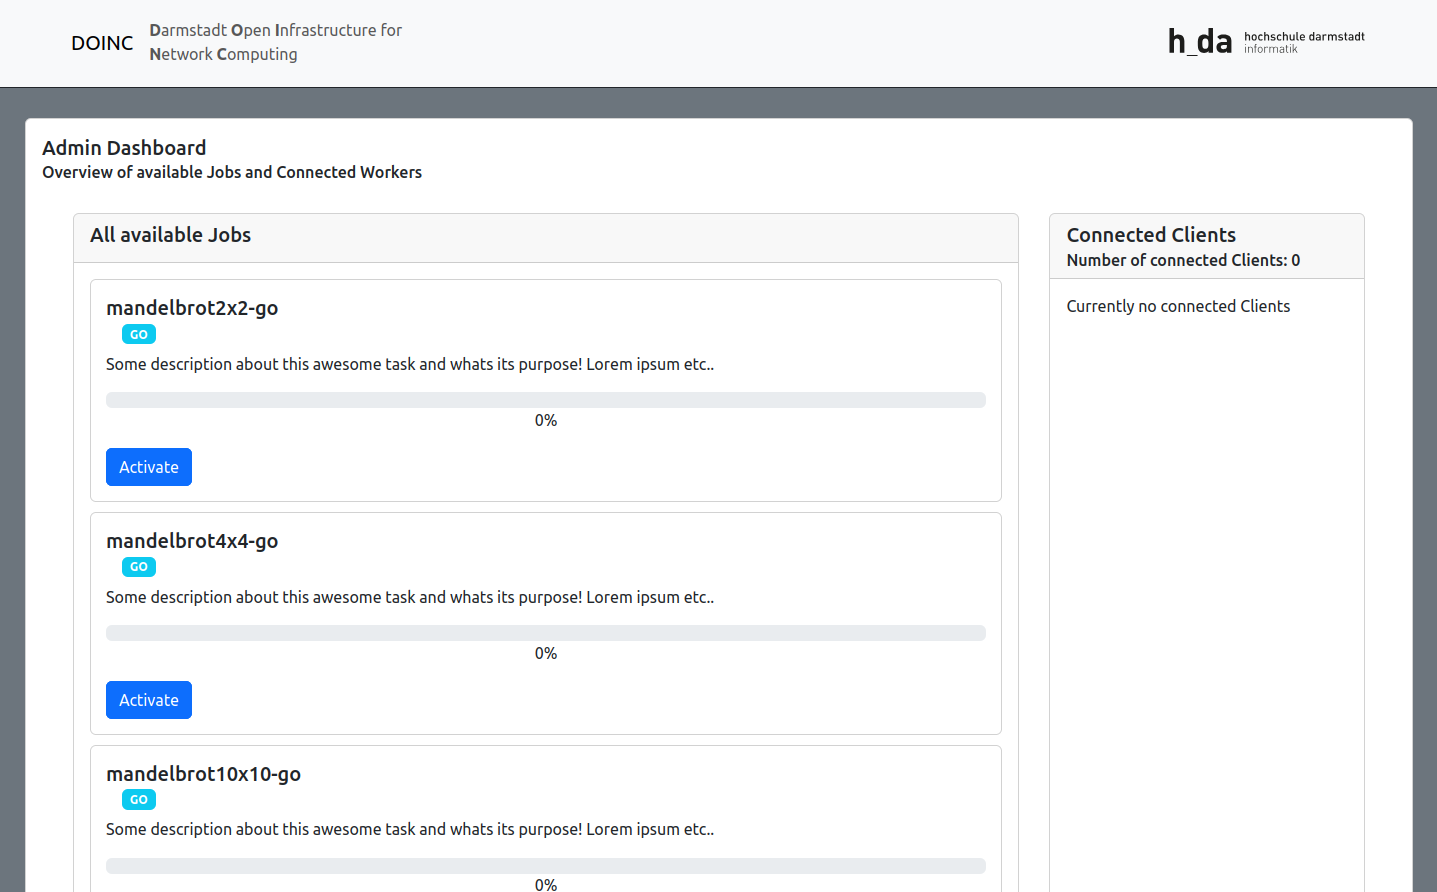
\includegraphics[width=.95\linewidth]{gfx/figures/active-job.png}
    }
    \caption{Frontend Dashboard Page}
    \label{fig:implementation:dashboard-page}
\end{figure}

On the left side of the \emph{Dashboard Page} is a component located to manage the Jobs of the platform. It holds a list of all existing Jobs and their current progress, displayed in figure \ref{fig:implementation:job-list}. Above this list of Jobs appears a new component when a Job is activated by an Administrator. Figure \ref{fig:implementation:active-job} displays a view of this active Job component on the left side. This component visualizes the progress of an active Job and displays the gathered results of complete Tasks in real-time. Additionally it provides an interface to interact with this Job. When a button of this interface is clicked, a corresponding \acs{HTTP} request, containing the Administrator's \ac{JWT}, is transmitted to the server. After all Tasks are completed and the state of the Job is \emph{DONE}, this component presents information about the total run time of the Job. On the right side is another component located that displays a list of all connected Workers also in real-time. This list contains information about the initialization progress as well as the harware and operating systm for each Worker with a active WebSocket connection to the Server. A view of this list is displayed in figure \ref{fig:implementation:active-job} on the right side.

\subsection{Client Page}
\label{subsec:implementation:client-page}

The \emph{Client Page} represents the logic for Workers and can be accessed by Workers or Administrators. When a client is accessing this web page the browser process becomes a participating Worker in the crowd computing platform. First the Worker establishes a WebSocket connection to the Server to recieve Job and Task data and to send Task results as described in section \ref{subsec:implementation:architecture:communication}. If this connection is successful the browser user agent of the Workers device is extracted and transmitted to the Server. When a Job is active or running the connected Worker is creating an independent browser thread - the WebWorker - and initializes the corresponding WebAssembly environment inside this WebWorker. Each Task that the Worker is receiving is forewarded for computing to this WebWorker. The performance and availabilty of the main browser thread, responsible for the \ac{UI} and WebSocket connection, is not affected by the processing of incoming Tasks, since the heavy WebAssembly computation is handled inside the separate WebWorker.

In the current state of the project the Worker is implemented to initialize and execute WebAssembly binaries complied from either C \& C++, Go or Python source code. The support of further WebAssembly targeting langues can be added effortless to this work, since the usage of WebWorker scripts is handled generic. To support specific programming languages each WebWorker script requires additional unique gluecode during the WebAssembly initialization process.

Figure \ref{fig:implementation:client-page} displays the view of the \emph{Client Page}. The component lists various information like the WebSocket connection status, the current actively supported Job and statistics about Tasks completed by the Worker.

\clearpage
\begin{figure}[htbp]
    \centering
    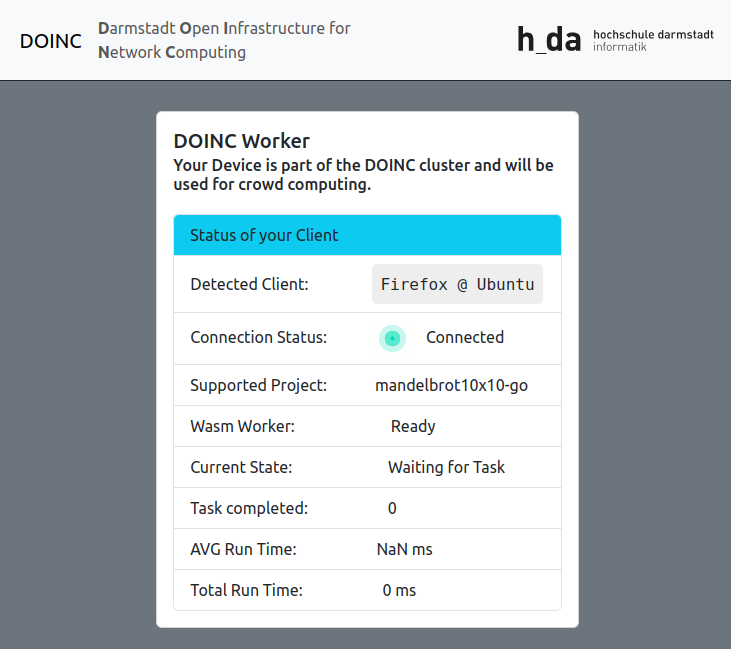
\includegraphics[width=0.95\textwidth]{gfx/figures/client-page.png}
    \caption{Frontend Client Page}
    \label{fig:implementation:client-page}
\end{figure}

\section{Benchmark}
\label{sec:implementation:benchmark}
As described in section \ref{sec:methodology:benchmark}, the visualization of the Mandelbrot set is used to benchmark the performance of the crowd computing platform in this work. The total run time of this Job, distributed among multiple Workers, is compared to native code execution of the same Job on a single device.

Since the Mandelbrot set represents a subset of complex numbers, it is visualized in a two-dimensional coordinate system representing the two-dimensional complex plane. The primary region of interest is located in an area bounded by $1$ to $-2$ on the X-axis (real numbers) and $1.5$ to $-1.5$ on the Y-axis (imaginary numbers). This area is partitioned into 100 equally sized sections, forming a 10x10 grid. Each grid tile represents the input arguments of a distinct Task. An additional Task computes the entire area of the Mandelbrot set at a lower resolution, resulting in a total of 101 unique Tasks for the visualization Job. Each of these Tasks produces a \ac{PNG} file visualizing its corresponding Mandelbrot set tile, utilizing the same color scheme as illustrated in Figure \ref{fig:methodology:mandelbrot}. Each Task computes the Mandelbrot condition for 9 million complex numbers $c$ within a 3000x3000 square region. Each of these 9 million $c$ is representing a pixel in the \ac{PNG} file generated by the Task. On Task completion the generated \ac{PNG} file is transmitted to the Server via the WebSocket connection and stored on the Server in a corresponding directory. After the Job is successfully completed an interactive Mandelbrot visualization becomes accessible via the Mandelbrot page in the Frontend.

The WebAssembly-compatible Go source code, which is executed by Workers during Task computation, is presented in \ref{app:code:mandelbrot2}. The corresponding native Go implementation, executed in comparission on a single device, can be found in \ref{app:code:mandelbrot3}.

\section{Challenges}
\label{sec:implementation:challenges}
what was difficult?
\begin{itemize}
    \item Hadel Input and Output
    \item Output as File (PNG)
    \item Prevent dublicate Task execution
    \item Minimize Communication
    \item Continue Stoped Job
    \item Implement system recovery
    \item load gluecode and wasm from third party in Webworker
    \item generic Job implementation
    \item generic handeling of different programming languages
\end{itemize}